\documentclass[10pt, conference]{IEEEtran}
%\documentclass[a4paper]{IEEEtran}
\renewcommand\IEEEkeywordsname{Keywords}

\ifCLASSINFOpdf

\else

\fi

\usepackage{graphicx}             % import, scale, and rotate graphics
\usepackage{subfigure}            % group figures
\usepackage{url}                  % facilitate linebreaking of URLs
\usepackage[T1]{fontenc}
\usepackage{nicefrac}             % write fractions in the text
\usepackage{indentfirst}          % indent the first paragraph
\usepackage[super, negative]{nth}
\usepackage{amsfonts}
\usepackage{amssymb}
\usepackage{multirow}
\usepackage{url}

\usepackage[dvipsnames,usenames]{color}
\usepackage{xspace}
\usepackage{balance}

\usepackage[latin1]{inputenc}     % use characters with accents in the source
\usepackage{moreverb}
\usepackage{amsmath}
\usepackage{xspace}
\usepackage{color}
\usepackage{paralist}             % to add in paragraphe enumerate list
\usepackage{booktabs}
\newcommand{\ed}[1]{\textsf{\textbf{[#1]}}}  %editorial comments
\newcommand{\dfn}[1]{\textit{#1}}            %introducing new terms
\newcommand{\revision}[1]{\textsf{\textbf{#1}}}
\newcommand{\co}[2]{#1 & \tiny{$\pm#2$}}     %intervalles de confiance

\newcommand{\yue}[1]{\textcolor{blue}{(\textbf{[Yue] }\textit{#1}})}

\graphicspath{{.}{./Pics/}}




% correct bad hyphenation here
\hyphenation{op-tical net-works semi-conduc-tor}


\begin{document}

\title{ns-3 Implementation of LISP and LISP-MN }

\author{Yue Li{$^{\ast}$}, Luigi Iannone{$^{\ast}$}, Benoit Donnet{$^{\dag}$}\\
$\ast$ Telecom ParisTech -- France\\
$\dag$ Universit\'e de Li\`ege, Montefiore Institute -- Belgium
}



\maketitle
%-----------------------------------------------------------------
\begin{abstract}
The \emph{Locator/Identifier Separation Protocol} (LISP) reconstructs the
current IP addressing space to improve the scalability and no interrupt mobility
issues. LISP Mobile Node (LISP-MN) is based on the basic LISP functionality to
provide seamless mobility across networks. The basic LISP architecture is
deployed on LISP Beta Network and LISP-Lab platform to offer the researchers a
realistic experimental environment, but both do not support LISP-MN. Some
simulation models with LISP extensions are implemented on various simulators,
but are unfortunately not open source. Providing a free and flexible simulation
model with the basic LISP architecture as well as the extensions so to help
researchers quickly test new LISP behaviors motivates our work. This paper
introduces the implementation of the basic LISP architecture model and LISP-MN
in ns-3. It also provides the evaluation results in mobility
scenario to validate the model and shows that, when the current proposal of
LISP-MN is behind a LISP-site, it has a very high delay during the handover
procedure.
\end{abstract}
%-----------------------------------------------------------------

  

\begin{IEEEkeywords}
	LISP, mobility, LISP-MN, ns-3, simulation.
\end{IEEEkeywords}

\IEEEpeerreviewmaketitle


%-< SECTION >--------------------------------------------------------------------
\section{Introduction}\label{sec:intro}

The \dfn{Locator/Identifier Separation Protocol} (LISP)~\cite{rfc6830} is
initially proposed to solve the scalability and flexibility issues of current
Internet architecture, since it decouples the \dfn{Routing Locators} (RLOCs,
i.e., an attachment point in the Internet topology) and \dfn{Endpoint
Identifiers} (EIDs, i.e., a communicating end-point). This allows the BGP
routing tables in the Internet core to only announce the globally routable RLOCs
whereas EIDs are only locally used within the LISP-sites. LISP is under
standardization at the IETF for about ten years and, with time, more and more
advantages are found such as: seamless mobility at terminal or in the Data
Center~\cite{saucez2016locator}, IPv6 transition and traffic
engineering~\cite{saucez2012designing}. In particular, the continuous
communication without interruption during the handover of terminals becomes a
hot topic recently~\cite{phoomikiattisak2016control}.

To test the various features of LISP, two LISP testbeds are built: LISP Beta
Network~\cite{lispbeta} and LISP-Lab platform~\cite{lisplab}. Unfortunately, both of
them only implement the basic LISP architecture and do not support mobility
functionality. Some platform-specific LISP implementations, such as
OpenLISP~\cite{phung2014openlisp}, Open Overlay Router (OOR)~\cite{LISPmob}, and
Cisco's implementation~\cite{CiscoIOS}, can provide realistic LISP evaluations
but lack the required flexibility for testing new and advanced LISP features.
% Further, a simulating environment for LISP would be valuable for researches as it would allow them to test, in a controlled and reproducible environment, the tomorrow LISP.
Thus, a simulating environment for LISP would be necessary and valuable for researches to improve LISP.
\ed{BD: better but should probably be rewritten a little bit.}\yue{Modified, better?} On
one hand, LISP has already been implemented in
ns-3~\cite{lezama2009implementation}, a widely used open-source simulator by
academic researchers and educational.  However, this implementation does not
support mobility.  On the other hand, LISP and mobility features are already
implemented in OMNET++~\cite{klein2012integration}. However, the source code is
not available online. To promote the development of LISP and as ns-3 gradually
shows the potential to take the momentum in network simulator
domain~\cite{rana2017implementation}, it highlights the importance to implement
LISP and its mobility extensions under ns-3. % and motivates our work.  
\ed{BD: last sentence unclear}\yue{Simplified, better?}

In this paper, we introduce the implementation of basic LISP functions and
mobility features on ns-3 by both modifying the existent ns-3 modules and
integrating new ones. Our implementation is validated through a mobility
scenario in which a terminal changes its attachment points while keeping the
communication up with the remote node. All the handover procedures are
transparent to the terminal.  However, the delay to receive the packets is high.

\ed{BD: you mention that the Omnet implementation is not open-source.  What
about yours?  If it is open-source,please provide a link in the paper to the
repo.}

The rest of the paper is organized as follows: Sec.~\ref{sec:lisp} reviews LISP
architecture, highlighting the LISP mobility mechanism; Sec.~\ref{sec:sim_model}
analyzes the design and implementation of our prototype, and afterwards,
Sec.~\ref{sec:evaluation} presents preliminary evaluation results of our
implementations. Sec.~\ref{sec:conclusion} concludes this paper by summarizing
its main achievements and discussing potential future works.

%-< SECTION >--------------------------------------------------------------------
\section{LISP Overview}\label{sec:lisp}


%-< SUB SECTION >--------------------------------------------------------------------
\subsection{Basic Architecture}\label{sec:archi}

LISP splits the current IP addressing space into two sub-spaces. One called EID
indicating the host identifier is locally used within a LISP-site. The other
one, called RLOC, represents the attachment point in the topology, i.e., the
border router, and is globally routable between LISP-sites on the Internet core.
The binding between EID and RLOC is called \dfn{mapping information} and is
stored in the \dfn{Mapping Distribution System} (MDS) consisting of \dfn{Map
Resolver} (MR) and \dfn{Map Server} (MS)~\cite{rfc6833}. The border router is in
charge of searching for the mapping information either in its own Cache or in
the MDS.  It then encapsulates the conventional IP packets into LISP packets and
forwards them out of the LISP-site on the Internet core.  This router is called
\dfn{Ingress Tunnel Router} (ITR).  On the other hand, routers receiving the
LISP packets and decapsulating them into traditional packets for the LISP-site
behind them are named \dfn{Egress Tunnel Router} (ETR). One usually refers to
both of them as \dfn{xTR}.


%-< SUB SECTION >--------------------------------------------------------------------
\subsection{LISP Mobile Node}\label{sec:lispMN}

The LISP Mobile Node (LISP-MN) implements a lightweight version of the standard xTR
functionality~\cite{mn14} supporting a node itself fast and seamless roaming% and being discovered in an efficient and scalable manner 
\ed{BD: unclear}\yue{Better?}. It can directly interact
with the MR to get the mapping information associated to the remote host, to which it communicates \ed{BD:
which remote host?}\yue{Is it clear now?}.
When a LISP-MN resides in a LISP-site, it is assigned an EID taken from the
site's EID-prefix as its RLOC, called \emph{Local RLOC} (\emph{LRLOC}) \ed{BD: I
think I understand the sentence but this is unclear}.
Thus, LISP-MN stores not only its permanent unique EID but also the LRLOC
and registers this mapping information to MS. The conventional IP packets
produced by the LISP-MN are encapsulated on itself using the permanent EID as
the inner source address and Local RLOC as the outer source address 
The encapsulated LISP packets are forwarded to xTR and encapsulated again by the
method of basic encapsulation of xTR. The procedure of packets being
encapsulated two times are called \emph{double encapsulation}.  \ed{BD:
this 1st encapsulation is unclear to me.  The EDI and LRLOC are used to
forward the packet to the xTR.  Then, the xTR encapsulates towards the distant
sites.  How this xTR knows the mapping of the distant site?  It is unclear
from this paragraph}.

%-< SUB SECTION >--------------------------------------------------------------------
\subsection{Mapping Cache Update Mechanisms}\label{sec:updateMechanisms}

When the ETRs change their LISP databases \ed{BD: never heard about the
databases before}, the only way that remote ITR can get the updated mapping
information is to re-request the mapping. Thus, Solicit-Map-Request (SMR) is
proposed to get the latest mapping.  \ed{BD: the broken English here makes the
sentence unclear.  SMR cannot be ``proposed''.}

Soliciting a Map-Request is used by ETRs to tell remote ITRs to update the
mappings they have cached in the Control Plane~\cite{rfc6830}. When the mappings
in the Database of ETR change, the ETR sends the Map-Requests with the SMR bit
set (called SMR message) for each RLOC in its Cache. A remote ITR that receives
the SMR message will send a Map-Request to the MR. During the sending SMR
message and receiving the new Map-Reply, the ITR continues to use the mapping
information previously cached, and that may cause the packet loss.

\ed{Bd: globally, this last subsection is unclear.}

%-< SECTION >--------------------------------------------------------------------
\section{Simulation Model}\label{sec:sim_model}

% -< SUB SECTION
% >--------------------------------------------------------------------
% \subsection{Description of ns-3}\label{subsec:descriptionns-3}
ns-3~\cite{ns3} is a popular and free discrete-event network simulator for networking research. % To be closer to the real implementation (in a real Operating System), easily include C-based implementation codes, ease debugging and reduce the cost on maintaining in a long term, C++ is prioritized to be the unique programming language for ns-3 \ed{BD: I personally don't think C++ is easy to debug\ldots  Is it really important to explain why C++ is used for coding in ns-3?  I'm not sure}. 
Besides, ns-3 offers the possibility to visualize the simulation instance so to allow the users to visually confirm the packets flow as they expect. Thus, we choose ns-3 to develop our LISP/LISP-MN simulator.


% -< SUB SECTION
% >--------------------------------------------------------------------
\subsection{Modifications to ns-3}
\label{subsec:modifyns-3}
% -< FIGURE
% >--------------------------------------------------------------------
\begin{figure*}[!t] \centering
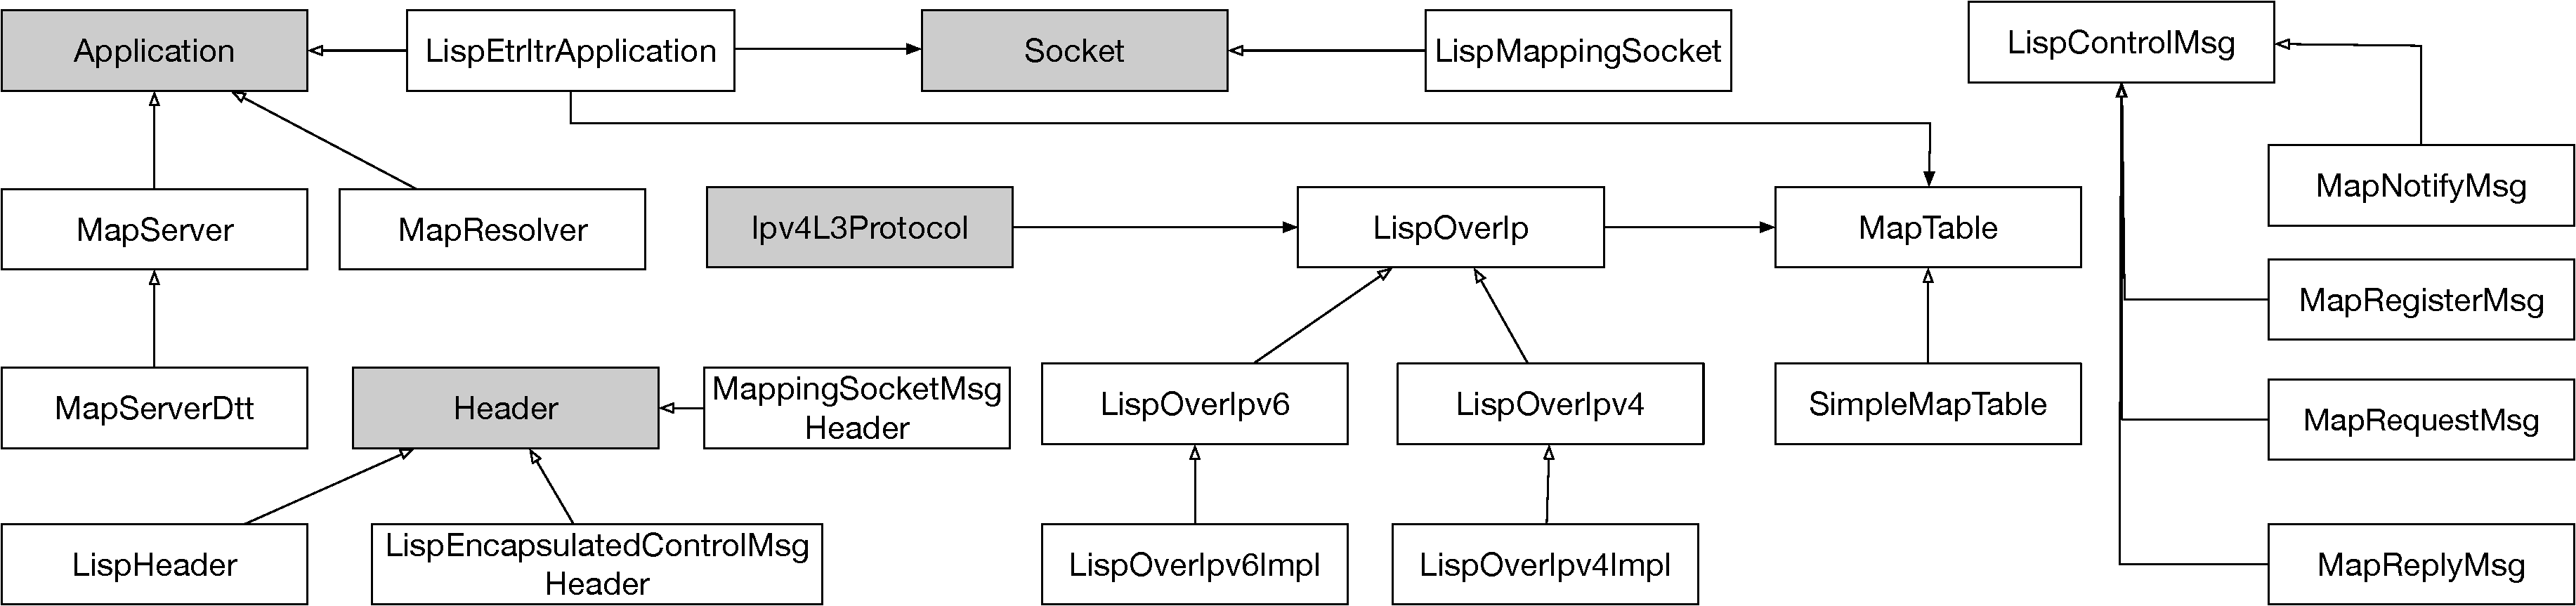
\includegraphics[width=\textwidth]{Pics/LISP-NS3-UML} \caption{UML diagram of
LISP/LISP-MN implementation. The solid arrow refers to a composition relation,
while the blank one refers to a inheritance relation.}
	\label{LISP-UML}
\end{figure*}
% -< END FIGURE
% >--------------------------------------------------------------------
Our implementation \ed{BD: should be open source.  Remind here the URL towards
the repo} is under ns-3.26 and based on LISP~\cite{ietf-lisp-rfc6830bis-03} and
LISP-MN standards~\cite{meyer-lisp-mn-16}. The main classes are shown in
Fig.~\ref{LISP-UML} in form of UML diagram. The blank blocks refer to the
classes that we added into ns-3, while darker blocks are classes already in
ns-3. As a design choice, we implement LISP/LISP-MN functionalities by modifying
and extending the \emph{internet} module of ns-3, instead of creating a new
independent module. The justification of this design is that LISP/LISP-MN and
legacy internet module have an interdependent relationship. However, this kind
of mutually dependent relationship between modules is not supported by ns-3.
Inspired by the OpenLISP design~\cite{saucez2009openlisp}, the Data Plane
implementation is in ``kernel space'' (i.e., ns-3 \emph{TCP/IP stack}) and the
Control Plane is implemented in ``user space'' (i.e., ns-3 \emph{Application}). 
The communication between LISP Data and Control Plane is ensured through a
dedicated socket (i.e., \emph{LispMappingSocket}) that inherits from the ns-3
\emph{Socket} class. It should be noted that our implementation only supports
IPv4 at time of  writing. The IPv6 support 
% (i.e. the implementation related to IPv6 such as \emph{LispOverIpv6Impl}) 
is still under construction.


% -< SUBSUB SECTION
% >--------------------------------------------------------------------
\subsubsection{Implementation of LISP Data Plane}\label{subsec:modifyInternet}
A LISP-compatible node (terminal or router) should be capable of determining
whether a packet should be passed to LISP-related procedure and retrieving the
associated mapping information if necessary. To this end, a new class called
\emph{LispOverIp} and its extended classes (refer to Fig.~\ref{LISP-UML}) are
added to ns-3 \emph{internet} module. This class is in charge of checking
whether necessary LISP-related operations (\texttt{NeedEncapsulation()},
\texttt{NeedDecapsulation()}) must be done, and of encapsulating conventional IP
packets (i.e., \texttt{LispOutput()}) as well as decapsulating LISP
packets(\texttt{LispInput()}). It also contains a smart pointer to the
LISP database and LISP cache.
Both data structures (store the EID-RLOC mapping information) are represented by
the class \emph{SimpleMapTable} that inherits from \emph{MapTable}. The
inheritance mechanism allows other users to implement their own implementation
of LISP database and cache. To support LISP functionalities, the \emph{Ipv4L3Protcol},
which is the IP layer implementation in ns-3, contains one \emph{LispOverIp}
object and \emph{Ipv4L3Protcol}'s packet transmission and reception procedures
are accordingly adapted.

To process outgoing packets, the adapted \texttt{send()} in \emph{Ipv4L3Protcol}
first verifies whether the \emph{LispOverIp} object is present. If yes, some
checks are then conducted to determine that this packet should be processed by
\texttt{LispOutput()} (to encapsulate the packets) or by conventional packet
transmission routine. For example, if both source and destination IP addresses
of this packet belong to the same network, the LISP-related process (e.g.,
encapsulation) is skipped and this packet is processed as in a non-LISP network.
Otherwise, EID-RLOC mapping information is searched from LISP cache and LISP
database on LISP-MN node. In case of a cache miss, the packet is dropped and
\texttt{SendNotifyMessage()} in \emph{LispOverIp} notifies, via a
\emph{LispMappingSocket} socket, the \emph{LispEtrItrApplication} that runs on
LISP-MN node. At the reception of the cache miss event from LISP Data Plane
(i.e., \emph{LispOverIp} object), \emph{LispEtrItrApplication} initiates a
Map-Request message to LISP mapping system. At the reception of the Map-Reply,
the received EID-RLOC mapping is inserted into LISP cache. It should be noted
that as an implementation choice, before the reception of Map-Reply message, all
transmitted packets with the required RLOC as destination are dropped. One can
also design a buffer to queue these packets and resend them once the required
mapping information is received via Map-Reply.
The advantage of such an implementation is to reduce the packet loss rate.

For an incoming packet, if the destination of this packet is the node itself,
the packet is processed by \texttt{LocalDelivery()} in \emph{Ipv4L3Protocol}.
Before passing to transport layer, \texttt{LocalDelivery()} checks if the packet
should be decapsulated. If yes, it is passed to \texttt{LispInput()}, in
which the packet is decapsulated and reinjected in the IP stack. If the received
packet destination is not this node, the packet is processed by patched
\texttt{IpForward()} method. This packet may be ended up with LISP encapsulation
procedure.


\subsubsection{Implementation of LISP Control Plane}\label{subsec:control-plane-impl}
The implementation of LISP Control Plane at least should provide ITR/ETR, MR,
and MS. In practice, ETR and ITR functionalities are usually placed on a same
router. In our implementation, they are included in the
\emph{LispEtrItrApplication} class. A ns-3 node that runs
\emph{LispEtrItrApplication} is a LISP-compatible router. It should be able to
communicate with \emph{LispOverIp} on the same node (e.g., inform about cache
miss) and other LISP-compatible routers (e.g., Map-Request/Map-Reply). To
support LISP-MN feature, \emph{LispEtrItrApplication} also communicates with
DHCP client application. For example, once a LISP-MN obtains an IP address from
the DHCP server, \emph{LispEtrItrApplication} receives the corresponding
EID-RLOC mapping and sends a Map-Register message~\cite{meyer-lisp-mn-16}.

A node that runs a \emph{MapServer} application is the MS in a LISP-supported
network. This class maintains a LISP database to store the EID-RLOC mapping
information, learned from Map-Register message at the initialization stage. In
current implementation, the role of MR is to receive the Map-Request message
from xTR and forward it to the MS.

% -< SUBSUB SECTION
% >--------------------------------------------------------------------
\subsubsection{Integration of TUN net interface card}\label{subsec:tundevice}
To support mobility, LISP-MN actually can be regarded as a small LISP-Site, in
which xTR functionalities and DHCP service are implemented, as well as
configured address of MR and MS. As a LISP-MN node, it has a static permanent
EID and dynamic RLOC assigned by the DHCP server. To differentiate with
conventional RLOC of xTR interface, such kind of RLOC is referred to as the
local RLOC (LRLOC). Different from conventional LISP node, at least two net
interface cards (NIC) are installed into LISP-MN. One is \emph{WifiNetDevice},
the other is a TUN type card. The DHCP client application runs on LISP-MN's
\emph{WifiNetDevice} and thus the LRLOC is allocated to this card. The permanent
EID is assigned to \emph{VirtualNetDevice} net card. We modify the node's
routing table so that each packet's inner header contains IP address on
\emph{TunNetDevice} and outer header contains IP address of \emph{WifiNetDevice}
as source address.

% -< SUBSUB SECTION
% >--------------------------------------------------------------------
\subsubsection{Integration of DHCP}\label{subsec:DHCP}
To support mobility within conventional LISP node, a modified DHCP client
application is integrated into ns-3 node. To be compatible with LISP
functionality, DHCP client application is modified. Once the DHCP client
receives an allocated IP address (i.e., LRLOC), it notifies the
\emph{LispEtrItrApplication} (i.e., LISP Control Plane) by sending a dedicated
message that contains the EID-LRLOC mapping. \emph{LispEtrItrApplication} is in
charge of populating the received mapping entry into LISP database. During the
mobility process, when wireless link is down, the DHCP client flushes the
LISP-MN database and populates the database again at the reception of a new
LRLOC.

% -< SECTION
% >--------------------------------------------------------------------
\section{Evaluation}\label{sec:evaluation}
We validate our LISP/LISP-MN implementation by conducting a simulation \ed{BD:
it is unclear to me how, at 1st glance, running a simulation can validate a
simulator (while you mention that in the Introduction)?} and providing a
preliminary performance evaluation of handover delay.
The topology used for the simulation is shown in Fig.~\ref{sim_scenario}.
\ed{BD: you could redraw this figure so that text appears larger}

%-< FIGURE >--------------------------------------------------------------------
\begin{figure}[!th]
	\centering
	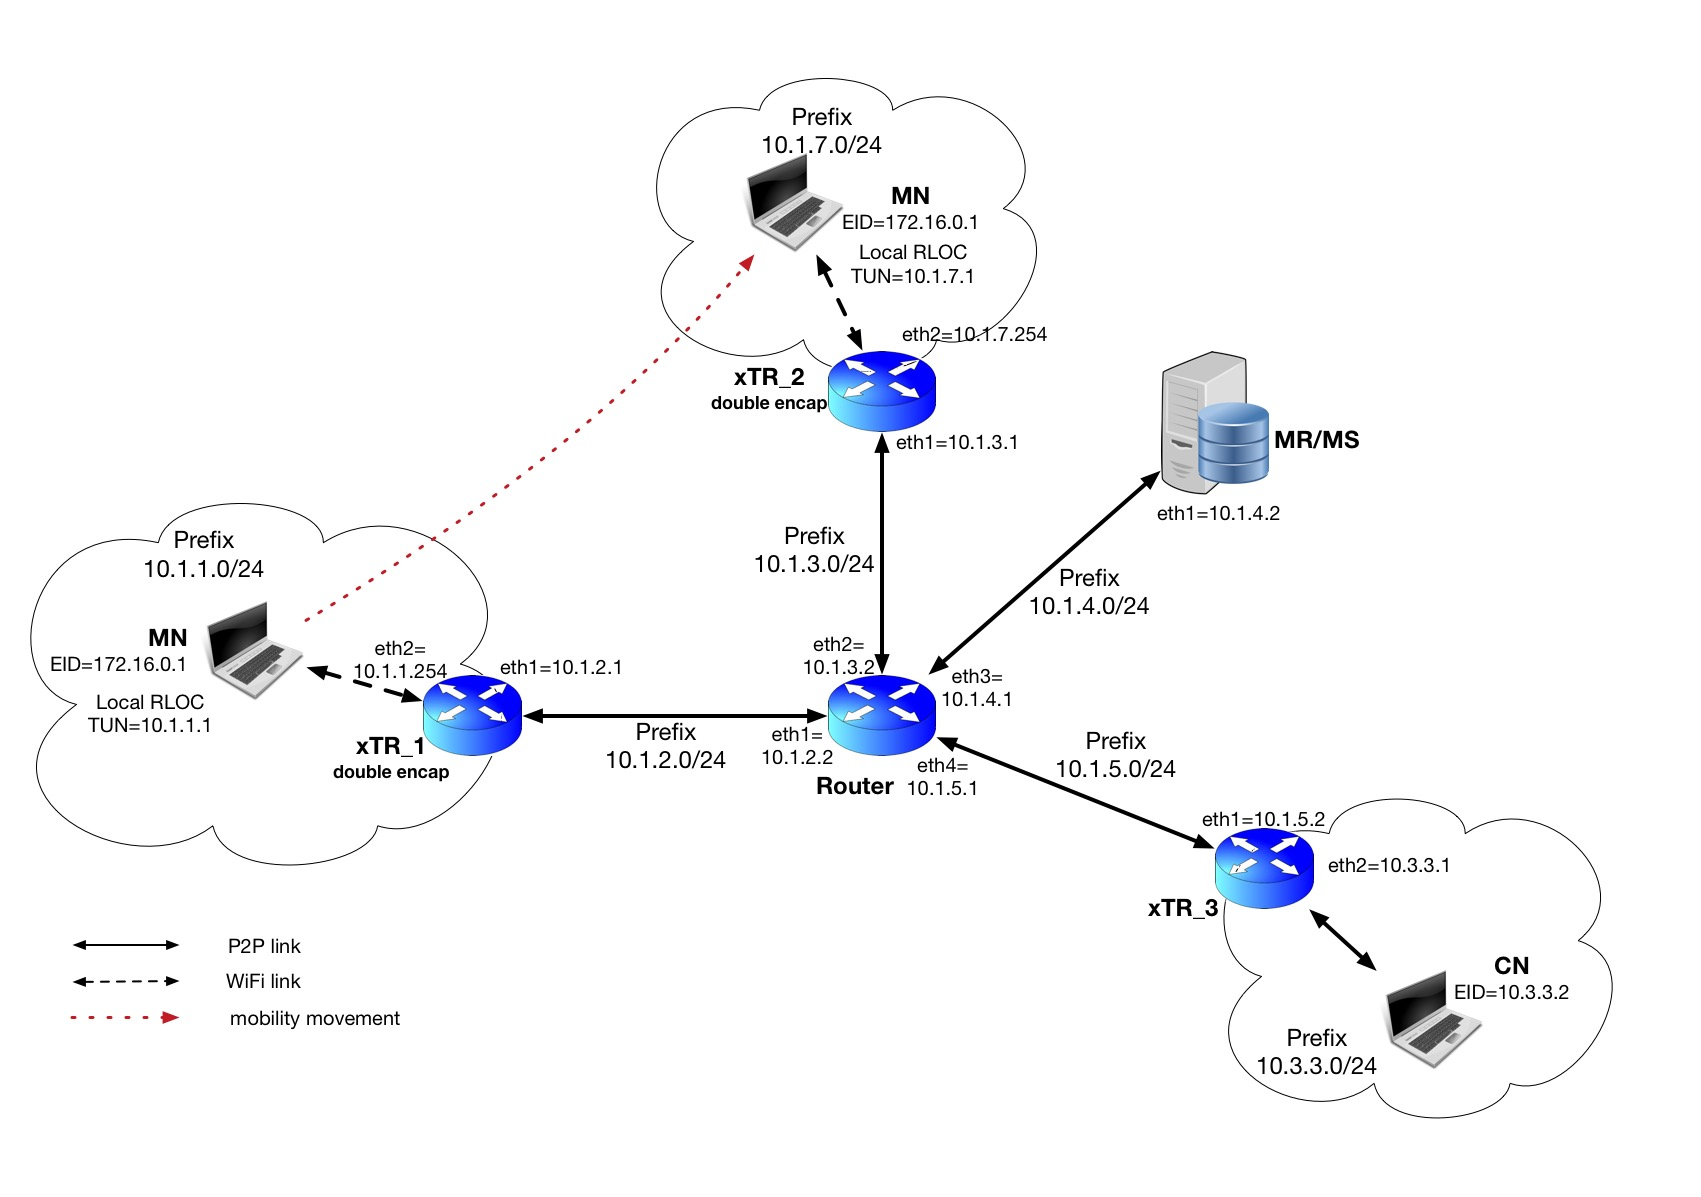
\includegraphics[width=0.5\textwidth]{Pics/mobility_through_subnets_2_encap_topo}
	\caption{LISP mobility simulation scenario for double encapsulation}
	\label{sim_scenario}
\end{figure}
%-< END FIGURE >--------------------------------------------------------------------

% -< SUB SECTION
% >--------------------------------------------------------------------
\subsection{Simulation Setup}\label{sec:setup}
In our simulation, a LISP-MN with permanent EID 172.16.0.1 is initially placed
in network 10.1.1.0/24. An \emph{echo} application on LISP-MN sends one packet
per second to a remote stationary node CN with EID 10.3.3.2, and the LISP-MN
moves into network 10.1.7.0/24 at speed of $7.07m/s$ \ed{BD: why that speed?}.
The distance between xTR\_1 and xTR\_2 is $170m$. LISP-MN node uses Wi-Fi to
connect to xTR\_1. At a certain moment during the move, the Wi-Fi link between
LISP-MN and xTR\_1 goes down, triggering so the handover procedure. Afterwards,
LISP-MN connects to xTR\_2 and reestablishes the communication with CN node. The
total simulation time is set to $45s$ and the DHCP procedure delay is set to
$1s$. We conduct many times of simulations \ed{BD: how many?  Did you average
the results?  If so, what is your confidence in the average (i.e., you
have to compute for each average the confidence interval)?} with the various
beacon interval of Wi-Fi channel in the range of $0.05s$ to $2s$ \ed{BD: why?}.


% -< SUB SECTION
% >--------------------------------------------------------------------
\subsection{Results}\label{sec:results}
As shown in Fig.~\ref{sim_schema}, when MN sends the packets to CN during the
simulation, it needs double encapsulation and the packet flow sequences are as
follows. The traditional IP packets with EID 172.16.0.1 as source address and
EID 10.3.3.2 as destination address are encapsulated by adding Local RLOC
10.1.1.1 as outer source address and RLOC 10.1.5.2 as outer destination address
after MN querying the mapping information to MR. The LISP packets are
encapsulated and forwarded to xTR\_1. The latter gets the mapping information
from MR and encapsulates the packets again by adding the RLOC 10.1.2.1 as the
outer source address and RLOC 10.1.5.2 as the outer destination address, then
sends the packets on Internet core. The xTR\_3 needs decapsulate the packets
twice after it receiving and verifying the packets, and finally sends to CN.
Once LISP-MN lost its Wi-Fi connection with xTR\_1, it needs a DHCP procedure
(consisting of DHCP Discover, DHCP Offer, DHCP Request and DHCP ACK) with xTR\_2
to get a new LRLOC 10.1.7.1 and then triggers LISP SMR to xTR\_3. After xTR\_3
getting new mapping information of <10.1.7.1, 10.1.3.1> and <172.16.0.1,
10.1.7.1>, the connection between LISP-MN and CN is re-established again.

%-< FIGURE >--------------------------------------------------------------------
\begin{figure}[!th]
	\centering
	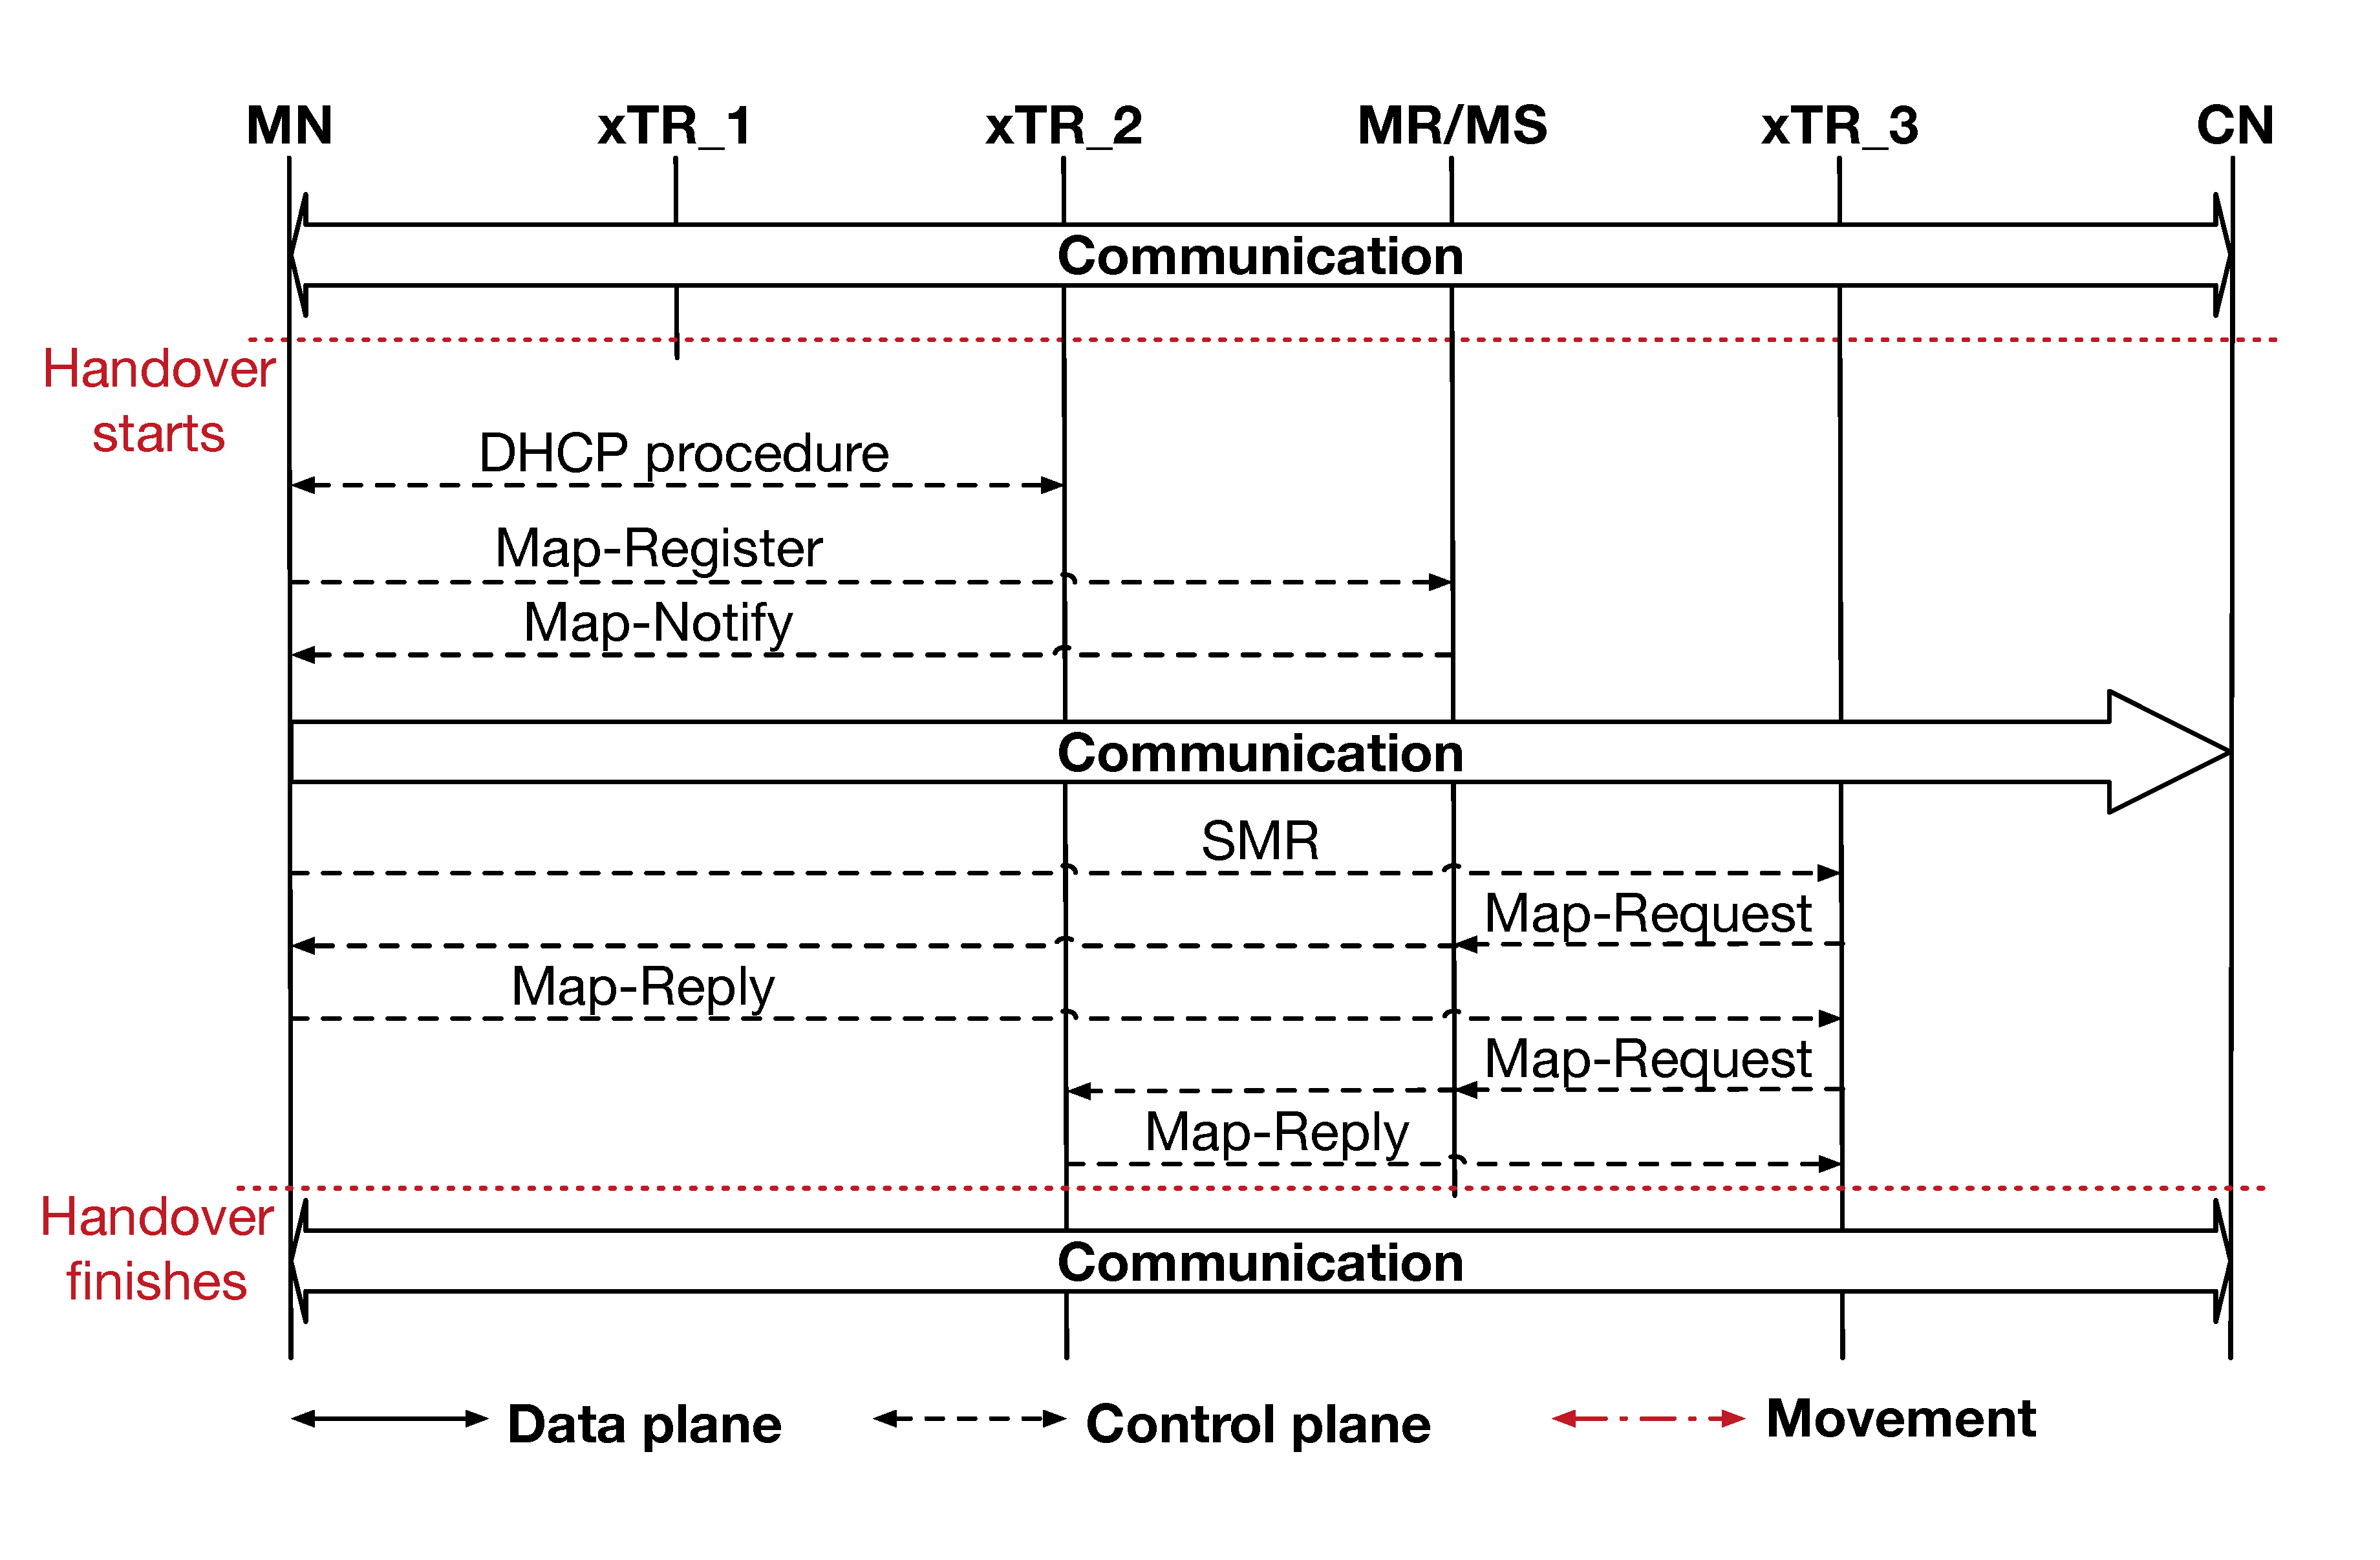
\includegraphics[width=0.5\textwidth]{Pics/Mobility_router_MN_supports_LISP_schema_SMR_simplify}
	\caption{Schema for LISP-MN mobility}
	\label{sim_schema}
\end{figure}
%-< END FIGURE >--------------------------------------------------------------------

The overall handover delay in this paper is defined at the moment that LISP-MN
sending DHCP Discover message to xTR\_2 and end up with xTR\_3 receiving the
last Map-Reply from xTR\_2 \ed{BD: unclear}. Precisely, it is made of three
parts:
the Wi-Fi association delay, the DHCP related delay, and LISP SMR delay:
\begin{equation}
    D_{overall} = D_{Wi-Fi}(BI) + D_{DHCP} + D_{SMR} \nonumber .
\end{equation}
where $D$ is the delay, $BI$ is Beacon Interval, subscriptions $Wi-Fi$, $DHCP$
and $SMR$ respectively refers to Wi-Fi association, DHCP procedure and LISP SMR.

After several runs \ed{BD: How much?} of the simulation, we observe
that the overall handover delay changes by the various beacon intervals, in particular the Wi-Fi
association delay depends on the different beacon intervals, whereas LISP SMR
procedure always cost around $3s$. To get the lower bound of overall handover
delay, we can ignore the Wi-Fi association delay when the beacon interval is
$500ms$, and the latency due to DHCP procedure is always $1s$. Thus, adopting
LISP-MN to conduct the host-based mobility takes at least $4s$. Compared to
current most stable solution for host-based IP mobility management MIPv6, which
latency including L2 and L3 in a real Wi-Fi testbed is around
$3.68s$~\cite{vassiliou2010analysis}, LISP-MN has a higher delay caused by the
double encapsulation mechanism introduced by LISP-MN behind LISP-Site.

During handover, CN can successfully receive packets from LISP-MN right after
DHCP procedure being accomplished, but LISP-MN cannot receive the packets from
CN until LISP SMR procedure is also finished. Thus, during DHCP procedure, all
bi-directional transmitted packets are lost. To improve the performance,
\cite{tang2017lisp} proposes a network-level LISP-MN solution, but has not
validated their proposals neither in simulation nor in testbed. Our ns-3
implementation can be used to realize them.

\ed{BD: I'm a little bit puzzled here.  I'm not sure what you really evaluate
in the sense that you rather provide a description of what happens during each
simulation run (i.e., message flow).  Do you have some quantification results
(for instance the latency variation over something)?}

% -< SECTION
% >--------------------------------------------------------------------
\section{Conclusion and future work}\label{sec:conclusion}
As a promising technology for the future Internet architecture, LISP attracts
more and more attention \ed{BD: ref?}. There exist some LISP implementations,
but they do not support LISP-MN or they are proprietary. Further, although measurements on
LISP-testbeds can provide real time performance, due to the complicated
topological structure, it is somewhat like a black box test which hinders us to
find the exact explanation for some results. This highlights the importance to
have an open source simulator for LISP in particular to support LISP-MN
functionality. In this paper, we present our implementation for LISP/LISP-MN
within ns-3, since the latter is a largely accepted simulator in networking
research. The simulation results show that our implementation works well, and
reveal the current LISP-MN proposal with a double encapsulation that has an high
level delay during handover procedure. Our simulator can be a perfect choice to
test the improvements of LISP-MN. 

There are two possible directions to support IP mobility in LISP: host-based
(i.e. LISP-MN) and network-based (i.e., xTR) mobility. We can compare the
performance between LISP double encapsulation described in this paper with only
host supporting LISP and only router supporting LISP leveraging our proposed
simulator. As Map-Versioning~\cite{rfc6834} is another Mapping Cache update
mechanism, we can also compare the performance between it and SMR that we
present in this paper by our simulator.

\ed{BD: this is a (very) short paper. I would suggest to shorten the conclusion}




% use section* for acknowledgment
\section*{Acknowledgment}
Research work presented in this paper is supported by the French Research Agency
under ANR-13-INFR-0009 LISP-Lab Project (www.lisp-lab.org) and benefited support
from NewNet@Paris, Cisco's Chair "{\sc Networks for the Future}" at Telecom
ParisTech (\url{http://newnet.telecom-paristech.fr}). Any opinions, findings or
recommendations expressed in this material are those of the author(s) and do not
necessarily reflect the views of partners of the Chair.     

% \vspace{2mm}
% \footnotesize{\emph{Acknowledgments:} Research work presented in this paper is supported by the French Research Agency under ANR-13-INFR-0009 LISP-Lab Project (www.lisp-lab.org) and benefited support from NewNet@Paris, Cisco's Chair "{\sc Networks for the Future}" at Telecom ParisTech (\url{http://newnet.telecom-paristech.fr}). Any opinions, findings or recommendations expressed in this material are those of the author(s) and do not necessarily reflect the views of partners of the Chair.}


{%\small
\balance
\bibliographystyle{ieeetr}
\bibliography{Bibliography}
}


\end{document}


